%%% Local Variables:
%%% mode: latex
%%% TeX-master: t
%%% End:

\newpage

\subsection{Class Diagram}

A class diagram in the Unified Modeling Language (UML) is a type of static structure diagram that describes the structure of a system by showing the system's classes, their attributes, operations (or methods), and the relationships among objects.
The following diagrams will show the class diagrams for the smart contracts.

\namedfigure
{!htbp}
{img:storageClsDig}
{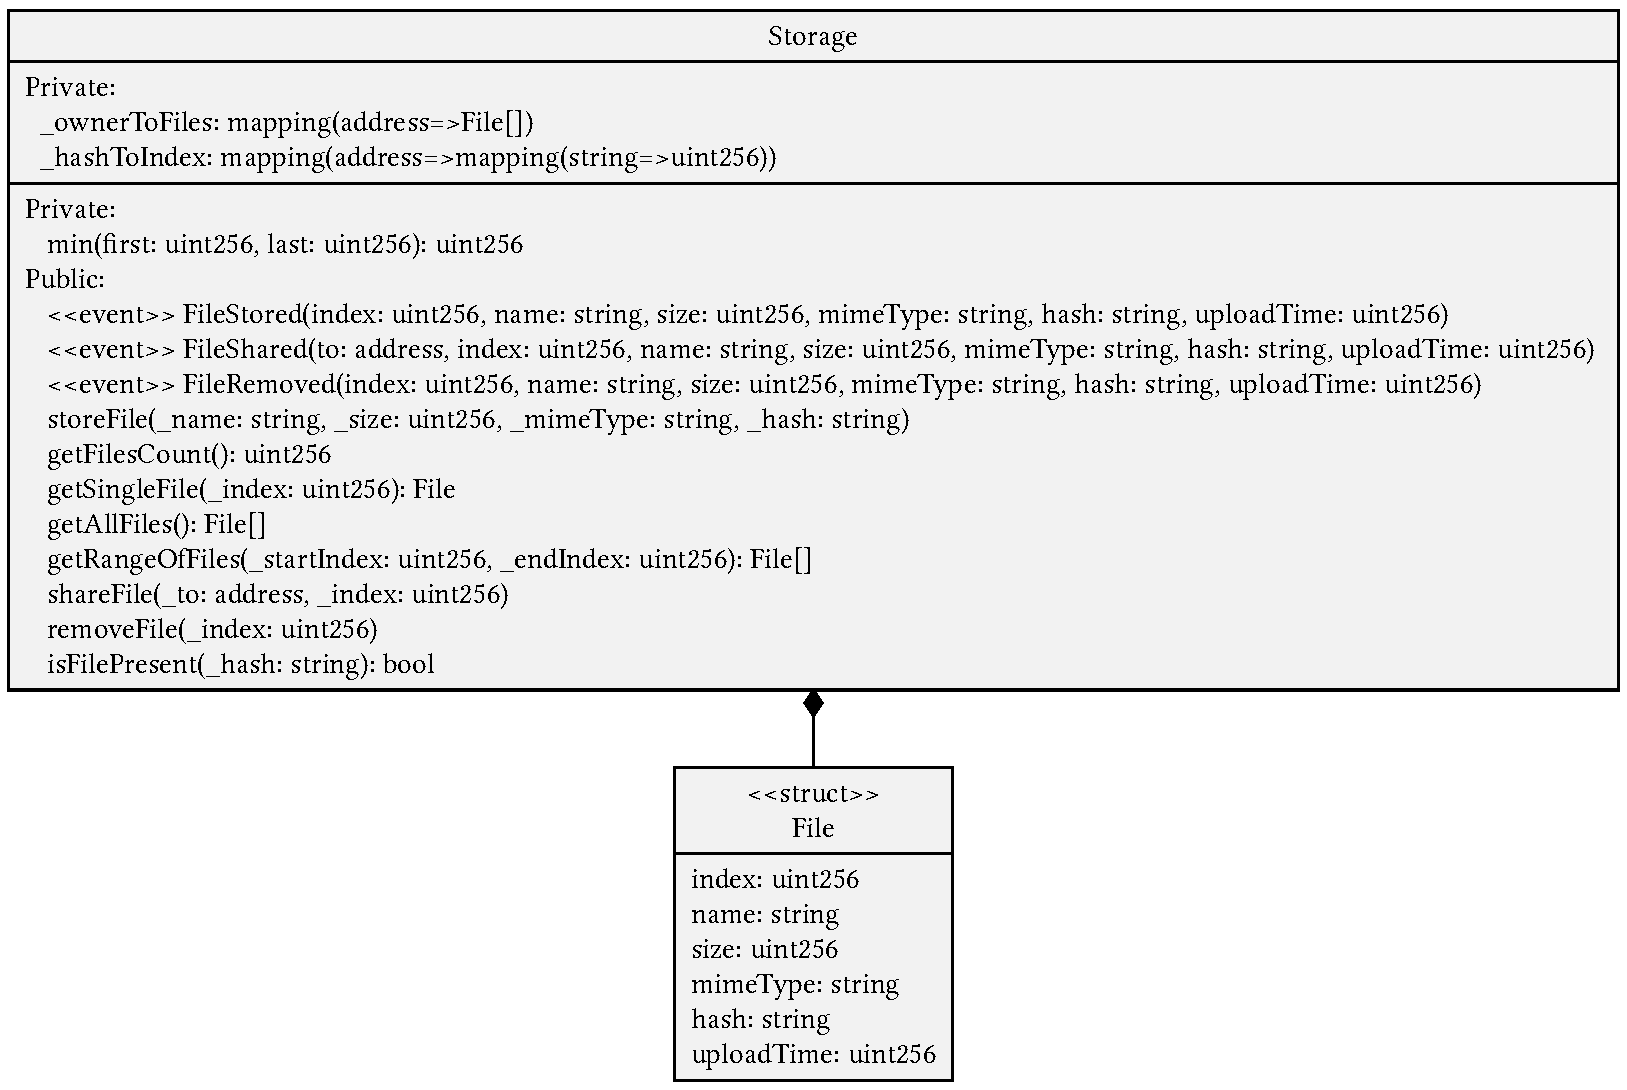
\includegraphics[width=\textwidth]{storage-class-diagram.pdf}}
{The smart contracts class diagram.}
